\documentclass{article}
\usepackage{amsmath,amssymb}
\usepackage{longtable}
\usepackage{graphicx}
\usepackage{float}
\usepackage[table]{xcolor}
\usepackage{amsmath}
\usepackage[english]{babel}
\usepackage{booktabs}
\usepackage{caption}
\usepackage{subcaption}
\usepackage{geometry}
\usepackage{array}
\usepackage{tabularx}
\usepackage{hyperref}
\usepackage{enumitem}
\usepackage[nottoc,numbib]{tocbibind}
\usepackage[titletoc,toc,page]{appendix}
\addtocontents{toc}{\protect\thispagestyle{empty}}

\geometry{a4paper, margin=1in}
\definecolor{TikTokBlack}{HTML}{040404}
\definecolor{TikTokPink}{HTML}{de8c9d}
\definecolor{TikTokRed}{HTML}{fe2858}
\definecolor{TikTokLightBlue}{HTML}{2af0ea}
\definecolor{TikTokDarkBlue}{HTML}{397684}

\begin{document}

% Center everything on the page
\begin{titlepage}
    \begin{center}

        % Logo and title
        
\includegraphics[width=0.1\textwidth]{./resources/logo.png} \\
        \vspace{0.5cm}
        {\Huge \textbf{TikTok-Brain}} \\[0.5cm]
        {\LARGE \textit{Lo-fi Prototyping and Usability Testing}} \\[2cm]

    \end{center}

    % Mission Statement
    \noindent
    \textbf{\textcolor{TikTokLightBlue}{\Large Mission Statement}} \\[0.3cm]
    \parbox{\textwidth}{
        \large
        To promote stair safety by leveraging the captivating power of video,
        delivering crucial safety messages in an engaging and distraction-free platform.
        % TikTok-Brain is both a community and competition platform that empowers individuals to take sustainable actions.
    } \\[1cm]

    % Value Proposition
    \noindent
    \textbf{\textcolor{TikTokBlack}{\Large Value Proposition}} \\[0.3cm]
    \parbox{\textwidth}{
        \large
        % Teamwork makes the green work.
        Delivering mesmerizing, randomized videos paired with essential safety advisories,
        TikTok-Brain simplifies social media to focus solely on enhancing personal safety without the clutter of likes, comments, or shares.
    } \\[1cm]


    % Problem / Solution Overview
    \noindent
    \textbf{\textcolor{TikTokRed}{\Large Problem / Solution Overview}} \\[0.3cm]
    \parbox{\textwidth}{
        \large
        Many individuals are unaware of the risks associated with inattentive stair use.
        Traditional safety messages often fail to engage audiences, leading to continued accidents and injuries.
        TikTok-Brain combines the engaging nature of short-form video content with critical safety messaging.
        By removing typical social media distractions,
        the app ensures that users receive and retain important information about walking safely on stairs.
    } \\[1.5cm]

    \begin{center}
        % Our Team
        \textbf{\textcolor{TikTokBlack}{\Large Our Team}} \\[0.5cm]

        % Team Photos and Names
        \begin{tabular}{ccc}
            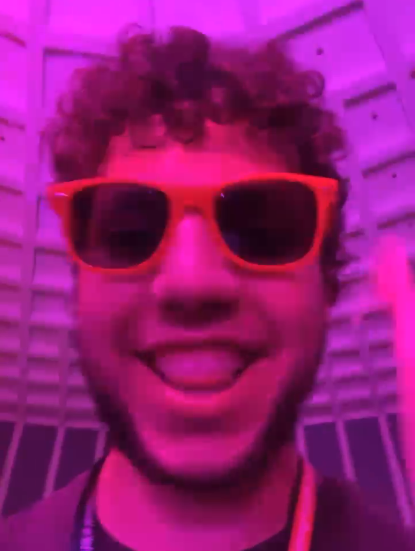
\includegraphics[width=0.2\textwidth]{./resources/ole.png} &
            
\includegraphics[width=0.2\textwidth]{./resources/markus.png} &
            
\includegraphics[width=0.2\textwidth]{./resources/diba.png} \\[0.3cm]
            Ole Einar Grundmann D493 & Markus Siegert D533 & Diba Zokai D583 \\
        \end{tabular}
    \end{center}
\end{titlepage}

\newpage
\tableofcontents
\newpage

\section{Introduction}
% Provide an introduction to the project, discussing the background, motivation, and objectives of your work. Describe the problem in more detail and explain why sustainability is crucial.
Distracted walking has become a significant safety concern, particularly on stairs where attention is crucial.
Traditional social media platforms, designed for high engagement,
inadvertently increase these risks by encouraging users to focus more on their screens than their surroundings.

TikTok-Brain is designed to counteract this issue by combining the engaging nature of video content
with crucial safety messages about walking safely on stairs.
This app simplifies the social media model: it removes likes, comments, and shares,
focusing solely on delivering safety-oriented content through mesmerizing, randomized videos paired with safety advisories.



% \section{Methodology}
% % This section explains the methodology used in your project. Break it down into subsections for clarity.
% The process began with an individual brainstorming phase,
% where each team member independently generated ideas.
% These ideas were then collectively refined using digital tools such as LaTeX, Gimp, and Krita,
% resulting in a diverse array of 25 to 30 potential concepts.

% To ensure our ideas were aligned with user needs and expectations,
% we proceeded to create and conduct a detailed survey comprising 20 questions,
% which was administered to 30 participants using Telekom Vote 2 and WhatsApp to reach out to the participants.
% The results helped constructing personas and refine our initial ideas.

% With a solid understanding of our user base,
% we evaluated the brainstormed ideas through a structured pro-contra analysis,
% taking into account the feedback and personas developed earlier.
% This phase of assessment was supported by Markdown and LaTeX,
% allowing us to narrow down our options to three final ideas.

% Subsequently, we moved to visually conceptualize these ideas through sketches and storyboards,
% utilizing Gimp, other graphic tools, and Kdenlive.
% This step was to visualize the sequence and flow of interactions,
% which were used for the later stages of prototyping.

% In a presentation to gather user feedback,
% participants evaluated the top three ideas from each of six groups, totaling 21 ideas.
% Each of the 25 attendees had two votes to allocate,
% allowing them to identify the concepts they found most compelling.
% This iterative process of development and refinement led to the selection
% of the most promising prototype based on its functionality and user feedback.

% The final stage of our project involved the creation of professional presentations and a comprehensive final report,
% crafted using PowerPoint and LaTeX. These documents provided a detailed overview of the project process,
% from the initial concept to the final evaluation of the prototype.



\section{Methods and Review}
To identify the exact problem and develop a solution, we used the double diamond method.
The double diamond method is originally a part of design thinking in business and has a user-oriented approach.
Therefore, one of its key elements is mockups and prototypes,
which are needed to get real user feedback in the ongoing development process.
The double diamond method has four phases, guiding the team from problem identification to a real solution.

The first phase is the 'Discover' Phase,
which is meant for gaining more insight into the problem and gathering information that may be essential for developing a solution.
In our project, the process began with an individual brainstorming phase, where each team member independently generated ideas.
These ideas were then collectively refined using digital tools such as
LaTeX, GIMP, and Krita, resulting in a diverse array of 30 potential concepts.
Moreover, we explained to each other why we created given ideas, always focusing on the expected user behavior.

Having finished the first phase, we moved straight into the second phase of the double diamond method.
In the 'Define' Phase, the gathered information was filtered, and the first possible solutions were reconsidered critically.
To ensure our ideas aligned with user needs and expectations, we created and conducted a detailed survey comprising 20 questions,
which was administered to 30 participants using Telekom Vote 2 and WhatsApp to reach out to the participants.
The results helped us construct personas and refine our initial ideas.
With a solid understanding of our user base, we evaluated the brainstormed ideas through a structured pro-contra analysis,
taking into account the feedback and personas developed earlier.
This phase of assessment was supported by Markdown and LaTeX, allowing us to narrow down our options to three final ideas.

As part of the third phase, the 'Develop' Phase, we started the actual design process.
All three ideas were laid down to focus on a simple and easy user experience, which was also the key aspect while designing.
Subsequently, we moved to visually conceptualize these ideas through sketches and storyboards,
utilizing GIMP, other graphic tools, and Kdenlive.
This step was aimed at visualizing the sequence and flow of interactions, which were used for the later stages of prototyping.

In a presentation to gather user feedback, participants evaluated the top three ideas from each of six groups, totaling 21 ideas.
Each of the 25 attendees had two votes to allocate, allowing them to identify the concepts they found most compelling.
This iterative process of development and refinement led to the selection of the most promising prototype
based on its functionality and user feedback.

In the last phase, the 'Delivery' Phase, we fully completed our most promising prototype
and made some improvements regarding the design and interactions of the prototype based on user feedback.
The final stage of our project also involved the creation of professional presentations and a comprehensive final report,
crafted using PowerPoint and LaTeX. These documents provided a detailed overview of the project process,
from the initial concept to the final evaluation of the prototype.

\subsection{Review}
The Double Diamand method is suitable for developing a lofi prototype. The individual phases and steps felt intuitive and promoted consistent progress. The method does not specify concrete tasks, but divides the entire development process into thematic phases. As a result, it requires minimal organisational time. The ‘Discover’ and ‘Define’ phases provide a good basis for inventing new creative ideas and rethinking and redefining old ones. Through these phases, you iteratively reflect on what the user wants and how the user acts. This allows ideas to be adapted, improved and reinvented. This consistently and proactively prevents a solution from being developed that does not appeal to the user.
To summarise, the Double Diamond method felt intuitive and very agile when developing a Lofi prototype. Since there is no strict procedure, but rather a generic approach, the Double Diamond method feels more like guidelines that teams can follow to develop a product or solution that is orientated towards the users.


\section{Results}
This chapter presents the progression from the already refined concept sketches to the final prototype,
detailing the design decisions, evaluations, and functionality development.

\subsection{Concept Sketches}
The top 3 of our concepts were:

\begin{enumerate}
    \item \textbf{Stair Master:}
        is a competitive stair-walking game designed for two players.
        Participants race against each other to see who can climb stairs the fastest while maintaining safety.
        The game emphasizes decision-making by introducing factors such as footwear selection and the use of the handrail.
        Players must strike a balance between speed and caution to succeed.
        The game aims to engage users with an entertaining approach to promoting stair safety
        while subtly educating them on the importance of safe practices.
    \item \textbf{StAIr:}
        is a humorous and interactive tool that generates AI made images of people falling down stairs.
        While this concept plays on humor, it serves as a reminder of the consequences of neglecting safety.
        The image-generation process integrates safety messages,
        ensuring users receive valuable advice while engaging with the entertaining visuals.
        By combining amusement with awareness, StAIr provides a unique way to stress the importance of staying vigilant on stairs.
    \item \textbf{TikTok-Brain:}
        Inspired by apps like TikTok,
        TikTok-Brain is a short-form video scroller that engages users with engaging,
        randomized videos displayed at the bottom of the screen.
        Safety messages are prominently displayed at the top, creating a dual focus that both entertains and educates.
        This concept eliminates traditional social interactions such as likes, comments, and shares,
        simplifying the experience to prioritize safety messages.
\end{enumerate}

\pagebreak

\begin{figure}[H]
    \centering
    \begin{subfigure}[t]{0.45\textwidth}
        \centering
        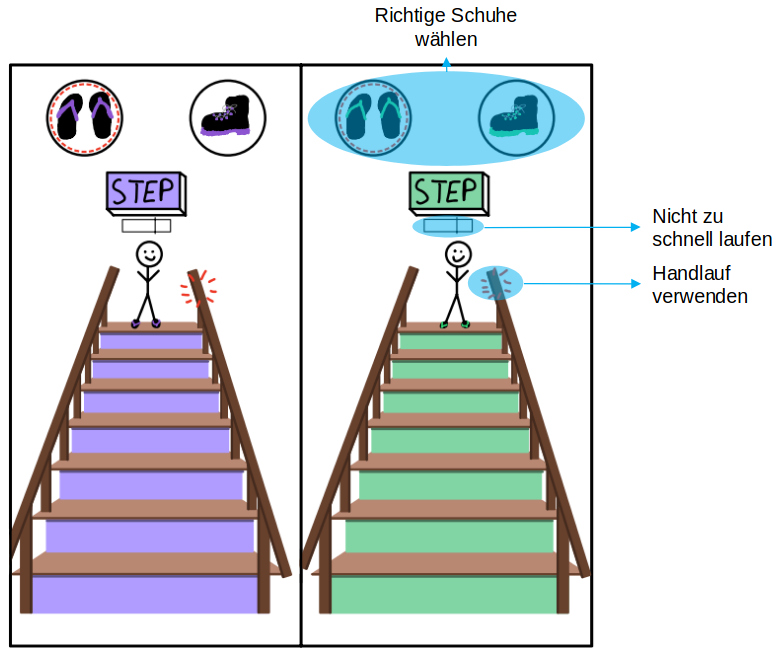
\includegraphics[width=\textwidth]{./resources/StairMaster_1.png}
        \caption{Tutorial Screen}
    \end{subfigure}
    \hfill
    \begin{subfigure}[t]{0.45\textwidth}
        \centering
        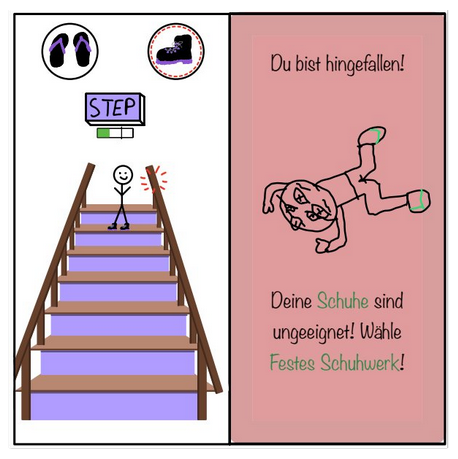
\includegraphics[width=\textwidth]{./resources/StairMaster_2.png}
        \caption{Death Screen}
    \end{subfigure}

    \vspace{0.5cm}

    \begin{subfigure}[t]{0.45\textwidth}
        \centering
        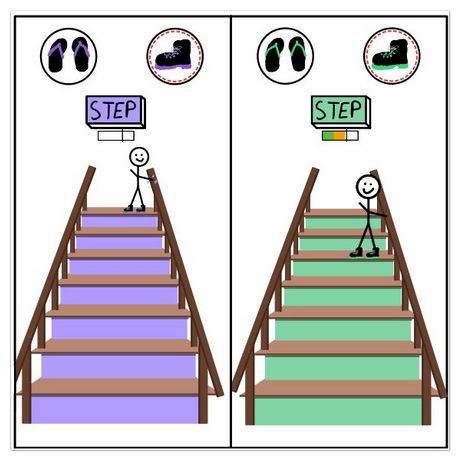
\includegraphics[width=\textwidth]{./resources/StairMaster_3.png}
        \caption{Progressing Gamestate}
    \end{subfigure}
    \hfill
    \begin{subfigure}[t]{0.45\textwidth}
        \centering
        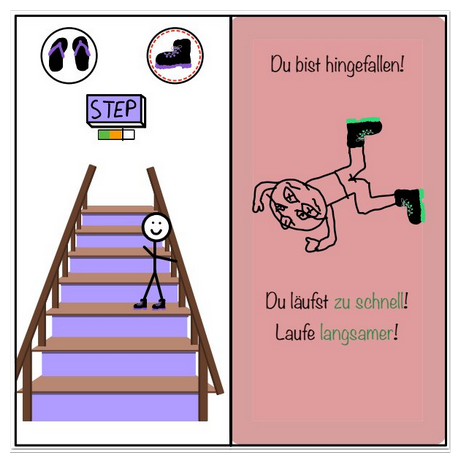
\includegraphics[width=\textwidth]{./resources/StairMaster_4.png}
        \caption{Second Death Screen}
    \end{subfigure}

    \vspace{0.5cm}

    \begin{subfigure}[t]{0.45\textwidth}
        \centering
        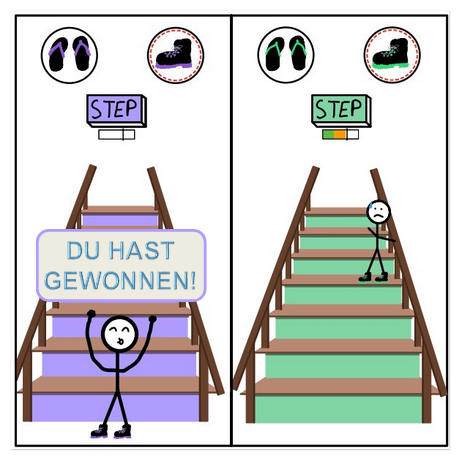
\includegraphics[width=\textwidth]{./resources/StairMaster_5.png}
        \caption{Winning Screen}
    \end{subfigure}

    \caption{Stair Master Game}
    \label{fig:StairMaster}
\end{figure}

\begin{figure}[H]
    \centering
    \begin{subfigure}[H]{0.8\textwidth}
        \centering
        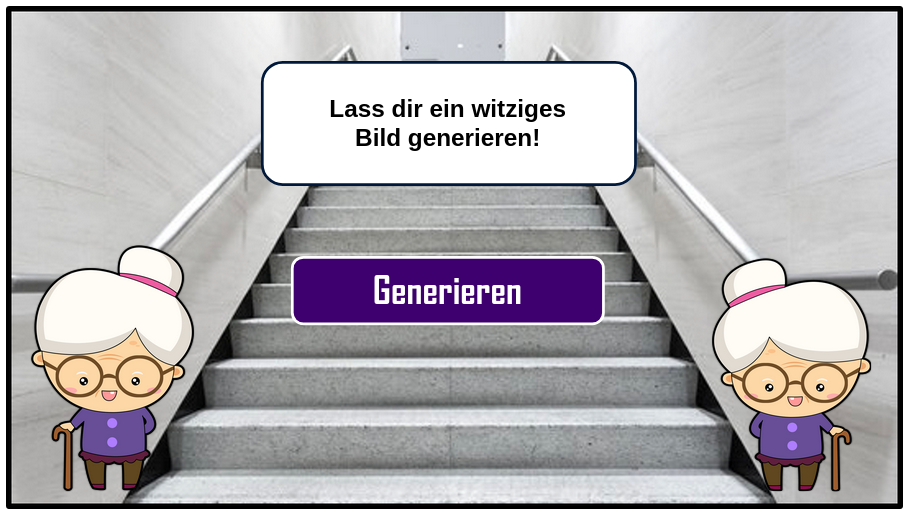
\includegraphics[width=\textwidth]{./resources/StairImgAI_1.png}
        \caption{Idle Screen}
    \end{subfigure}
    \hfill
    \begin{subfigure}[H]{0.8\textwidth}
        \vspace{3mm}
        \centering
        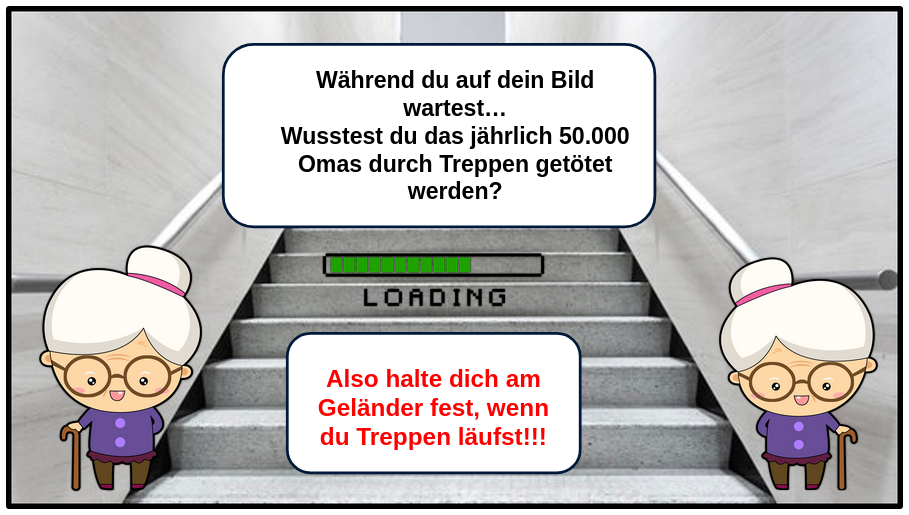
\includegraphics[width=\textwidth]{./resources/StairImgAI_2.png}
        \caption{Loading Screen}
    \end{subfigure}
    \hfill
    \begin{subfigure}[H]{0.8\textwidth}
        \vspace{3mm}
        \centering
        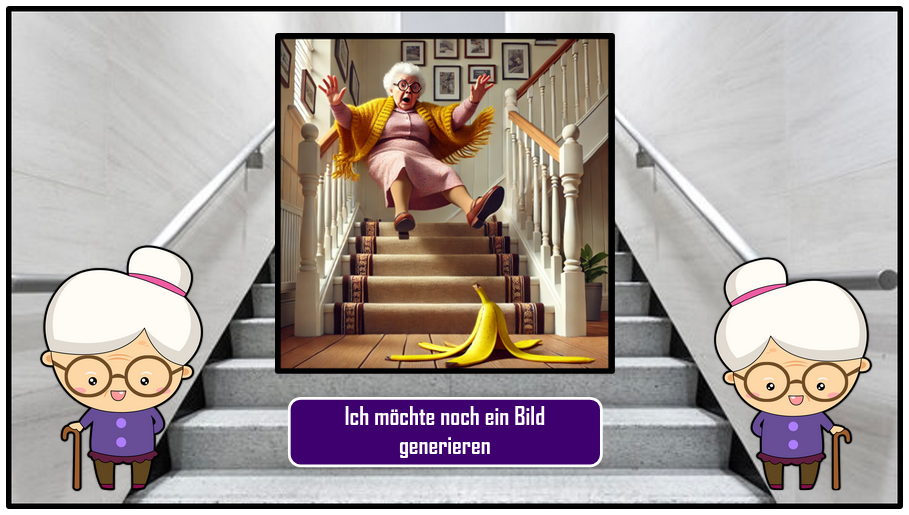
\includegraphics[width=\textwidth]{./resources/StairImgAI_3.png}
        \caption{Image presentation Screen}
    \end{subfigure}
    \caption{StAIr AI Image Generation}
    \label{fig:StairImgAI}
\end{figure}

\begin{figure}[H]
    \centering
    \begin{subfigure}[t]{0.45\textwidth}
        \centering
        
\includegraphics[width=\textwidth]{./resources/StairTikTokBrain_1.png}
        \caption{Video before Swipe}
    \end{subfigure}
    \hfill
    \begin{subfigure}[t]{0.45\textwidth}
        \centering
        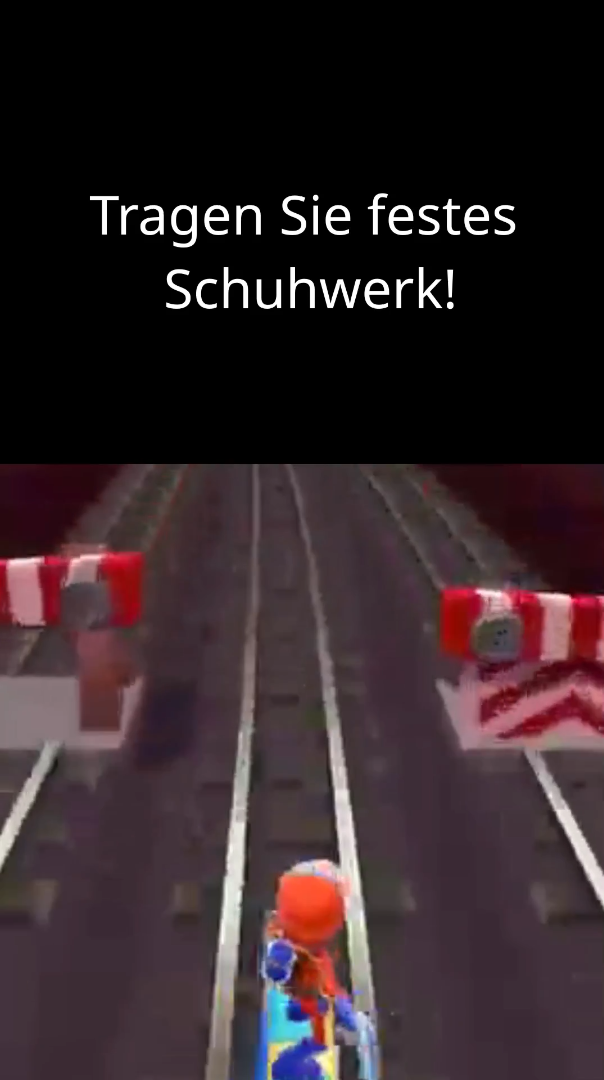
\includegraphics[width=\textwidth]{./resources/StairTikTokBrain_2.png}
        \caption{Video after Swipe}
    \end{subfigure}
    \caption{TikTok-Brain}
    \label{fig:StairTikTokBrain}
\end{figure}


\subsection{Selected Concept Designs}

This section draws from pro-con analysis tables derived from user feedback collected in earlier surveys.
It details the advantages and drawbacks of the designs for Stair Master, StAIr, and TikTok-Brain.
The feedback-driven tables offer essential insights into user preferences and engagement,
helping to explain the selection process and potential impact of each design on promoting safety awareness.
This evaluative approach emphasizes the user-centered design process
and highlights the importance of empirical feedback in refining and finalizing the concept designs.

In addition to the survey, a presentation followed by a voting session was conducted,
where Stair Master accomplished 1 vote, StAIr accounted 2 votes, and TikTok-Brain achieved 11 votes.
Having 22\% of the total votes positioned TikTok-Brain as the most favored concept among all 21 design concepts presented.

\setlist[itemize]{topsep=3pt, parsep=0pt, leftmargin=1em}
\begin{table}[H]
    \centering
    \textbf{\textcolor{TikTokBlack}{\large Stair Master Game (1 vote)\strut}}\par
    \renewcommand{\arraystretch}{1.5}
    \setlength{\tabcolsep}{12pt}
    \begin{tabularx}{\textwidth}{|>{\centering\arraybackslash}X|>{\centering\arraybackslash}X|}
        \hline
        \cellcolor{TikTokRed}\textbf{Pros} & \cellcolor{TikTokLightBlue}\textbf{Cons} \\
        \hline
        \vspace{-4mm}
        \begin{itemize}
            \item The majority enjoys playing minigames
            \item Social Gaming Interest
            \item Gaming Engagement
        \end{itemize}\nointerlineskip &
        \vspace{-4mm}
        \begin{itemize}
            \item Does not catch much interest
            \item Few positiv feedback
        \end{itemize}\nointerlineskip \\
        \hline
    \end{tabularx}
    \caption{Pro + Con analysis for Stair Master}
\end{table}

\begin{table}[H]
    \centering
    \textbf{\textcolor{TikTokBlack}{\large StAIr AI Image Generator (2 votes)\strut}}\par
    \renewcommand{\arraystretch}{1.5}
    \setlength{\tabcolsep}{12pt}
    \begin{tabularx}{\textwidth}{|>{\centering\arraybackslash}X|>{\centering\arraybackslash}X|}
        \hline
        \cellcolor{TikTokRed}\textbf{Pros} & \cellcolor{TikTokLightBlue}\textbf{Cons} \\
        \hline
        \vspace{-4mm}
        \begin{itemize}
            \item Humor Preference
            \item Catches attention because of AI use
            \item Simple User-Interface
        \end{itemize}\nointerlineskip &
        \vspace{-4mm}
        \begin{itemize}
            \item Humor is subjective
            \item Potential Insensitivity
            \item Attention may only focus on AI
        \end{itemize}\nointerlineskip \\
        \hline
    \end{tabularx}
    \caption{Pro + Con analysis for StAIr}
\end{table}

\begin{table}[H]
    \centering
    \textbf{\textcolor{TikTokBlack}{\large Stair TikTok-Brain (11 votes)\strut}}\par
    \renewcommand{\arraystretch}{1.5}
    \setlength{\tabcolsep}{12pt}
    \begin{tabularx}{\textwidth}{|>{\centering\arraybackslash}X|>{\centering\arraybackslash}X|}
        \hline
        \cellcolor{TikTokRed}\textbf{Pros} & \cellcolor{TikTokLightBlue}\textbf{Cons} \\
        \hline
        \vspace{-4mm}
        \begin{itemize}
            \item High Engagement with Memes and Humor
            \item Everyone spends time on short-form streamer daily
            \item Clear Warning Placement
        \end{itemize}\nointerlineskip &
        \vspace{-4mm}
        \begin{itemize}
            \item Lower Engagement with Short-form Video
            \item Attention may only focus on videos
        \end{itemize}\nointerlineskip \\
        \hline
    \end{tabularx}
    \caption{Pro + Con analysis for TikTok-Brain}
\end{table}

\begin{figure}[H]
    \centering
    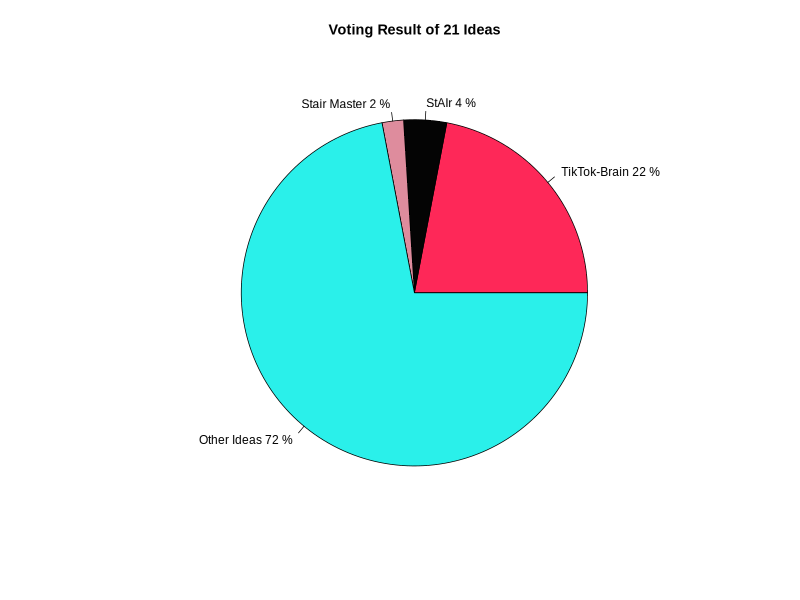
\includegraphics[width=\textwidth]{./resources/ideas_distribution.png}
    \caption{Presentation Voting Results}
    \label{fig:system-overview}
\end{figure}

\subsection{Prototyping}

We selected TikTok-Brain as the final design concept because it aligns strongly with user feedback,
engagement potential, and our core objective of promoting safety awareness.
This decision was informed, as already mentioned in the previous section,
by a thorough pro-con analysis based on user feedback from earlier surveys
and validated by a voting session involving all 21 design concepts.

\pagebreak

\begin{figure}[H]
    \centering
    \begin{subfigure}[H]{0.9\textwidth}
        \centering
        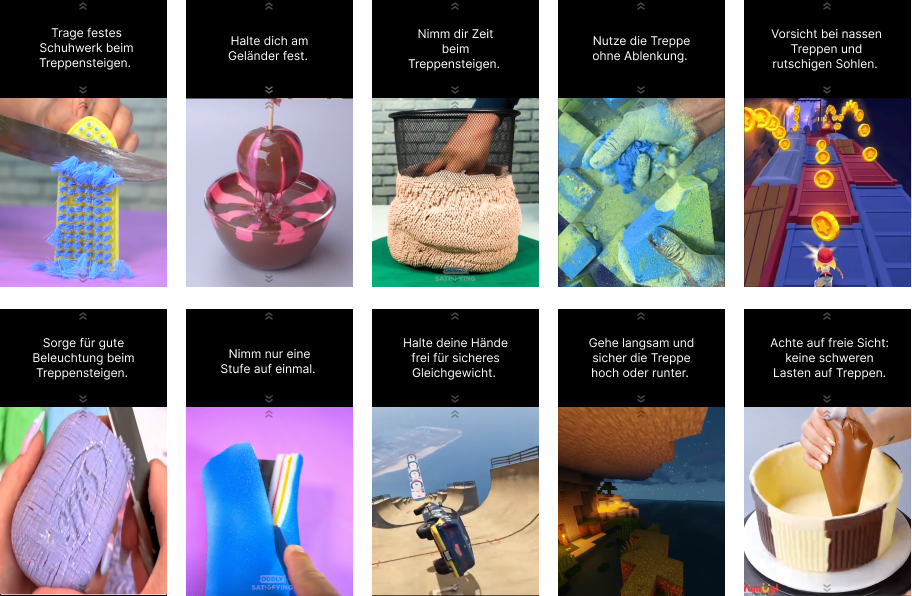
\includegraphics[width=\textwidth]{./resources/storyboard.png}
        \caption{Storyboard}
    \end{subfigure}
    \begin{subfigure}[H]{0.9\textwidth}
        \vspace{3mm}
        \centering
        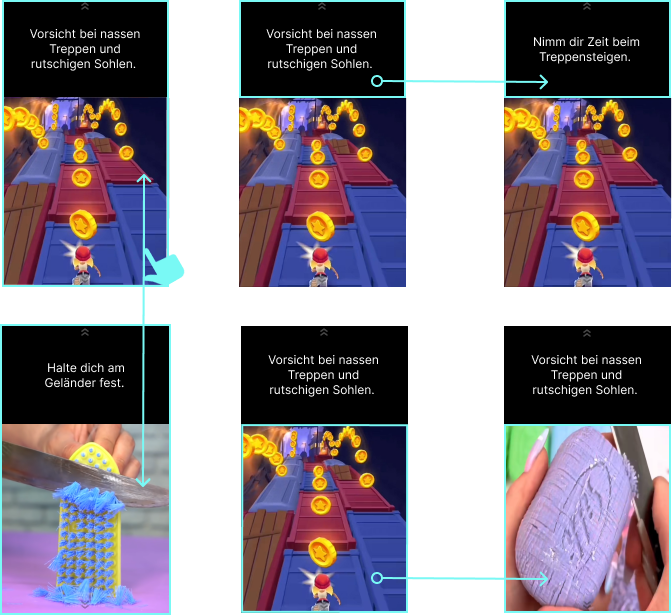
\includegraphics[width=\textwidth]{./resources/full-system.png}
        \caption{User Flow}
    \end{subfigure}
    \caption{Lo-fi Prototype of TikTok-Brain}
    \label{fig:prototype}
\end{figure}

% \begin{figure}[H]
%     \centering
%     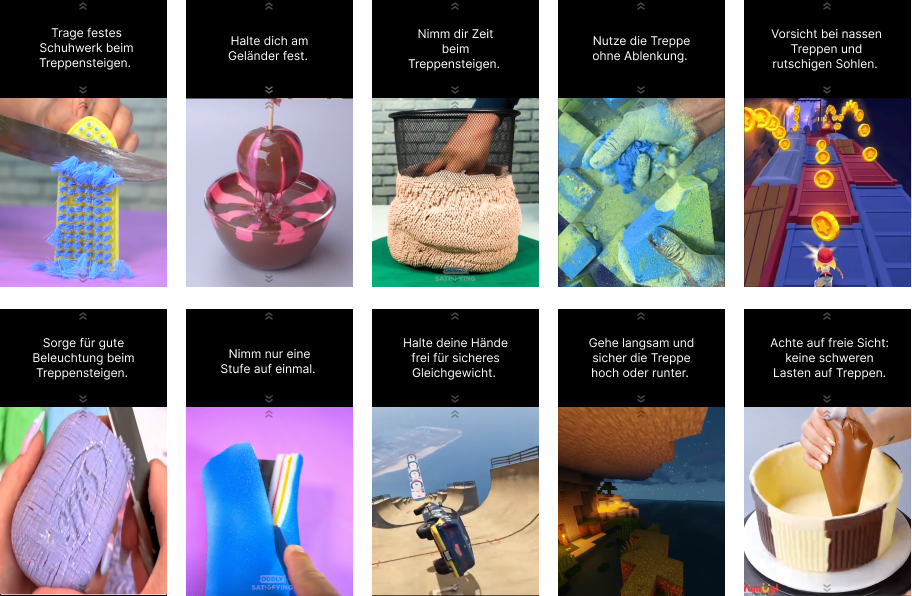
\includegraphics[width=\textwidth]{./resources/storyboard.png}
%     \caption{Lo-fi Storyboard of TikTok-Brain Platform Interactions}
%     \label{fig:storyboard}
% \end{figure}

% \begin{figure}[H]
%     \centering
%     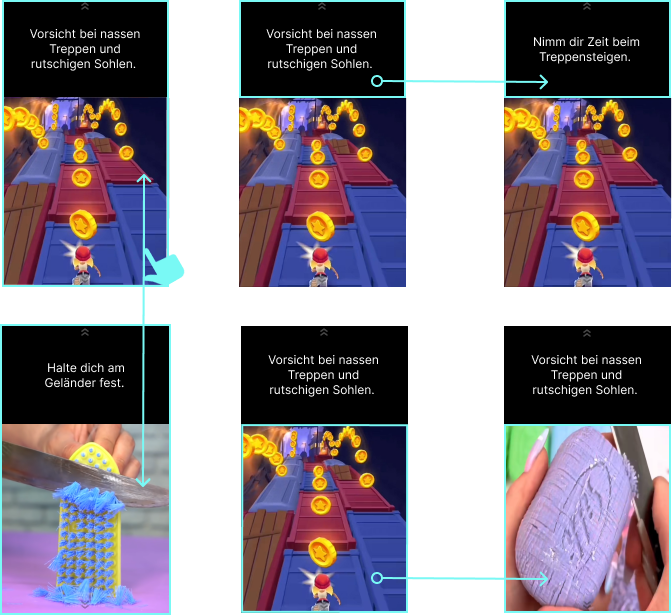
\includegraphics[width=\textwidth]{./resources/full-system.png}
%     \caption{Lo-fi Prototype of TikTok-Brain Platform Example Views}
%     \label{fig:system-overview}
% \end{figure}

\begin{table}[H]
    \centering
    \renewcommand{\arraystretch}{1.5}
    \setlength{\tabcolsep}{12pt}
    \begin{tabularx}{\textwidth}{|l|X|X|}
        \hline
        \cellcolor{TikTokRed}\textbf{Component} & \cellcolor{TikTokBlack}\textbf{\textcolor{white}{Description}} & \cellcolor{TikTokLightBlue}\textbf{Functionality} \\
        \hline
        Video Display Area & Fullscreen area to show videos. & Displays a single video at a time, taking up the bottom part of the screen. \\
        \hline
        Swipe Navigation & Gesture-based navigation for moving through videos. & Swiping up loads the next video; swiping down loads the previous video. \\
        \hline
        Random Video Loader & Logic that fetches a random video to display. & Randomly selects and loads a video from the video pool whenever a new video is required. \\
        \hline
        Text Overlay Area & Area at the top of the screen for text that accompanies each video. & Displays a random line of text (e.g., a phrase or quote) that’s paired with the video. \\
        \hline
        Video-Text Randomizer & Logic that pairs random videos with random text. & Ensures that each video is matched with a different text overlay each time it appears, maintaining freshness. \\
        \hline
        Interface Background & Background color or visual design behind the video display. & Provides visual consistency or mood but stays unobtrusive to keep focus on video and text content. \\
        \hline
        Loading Indicator & Small icon or animation that shows when new content is being loaded. & Briefly appears when the app fetches a new random video or reloads the feed. \\
        \hline
        No Interaction Buttons & No buttons for like, comment, or share, emphasizing simplicity. & Only swipe gestures are recognized; no additional UI elements for social interactions. \\
        \hline
        Error Handling Display & Fallback message or visual when loading fails. & Displays an error message if a video fails to load, with a prompt to restart the application. \\
        \hline
        Auto Swipe Animation & Animation that mimics a swipe if there’s no interaction for a while. & After a set period of inactivity, automatically performs a swipe animation to move to the next video, keeping the experience engaging. \\
        \hline
    \end{tabularx}
    \caption{Functionality of Design Interface Components}
\end{table}

\section{Project Report}
\subsection{Lessons Learned}
Throughout the TikTok-Brain project, there have been several valuable insights that will influence future work practices.
The use of iterative design and continuous user feedback have greatly helped to improve our concept
and demonstrated that early and frequent user involvement leads to more effective solutions.
The structured approach for the generation of ideas,
starting from individual brainstorming before moving to collective refinement,
has shown how the combination of independent thinking with collaborative evaluation
can create more diverse and innovative concepts.
A particularly valuable lesson was the importance of simplification:
by removing traditional elements of social media such as likes and comments,
we have created a more focused user experience that better serves our main goal of promoting security.
The progresson from survey-based research to persona development, followed by a structured pro-contra analysis,
has provided a solid framework for the decision-making process which can be applied to future projects.
We have also learned that even seemingly simple applications benefit from in-depth usability tests,
as user interactions often reveal unexpected insights into interface design and content delivery.
The project highlighted the challenge of balancing engagement with educational content
and taught us that entertainment and learning are not neccessarily mutually exclusive when properly integrated.
Furthermore, the experience of working with various digital tools (LaTeX, Gimp, Krita)
has emphasized the importance of choosing suitable technologies for different phases of any project.
Moving forward, the creation of detailed documentation throughout the development process,
and not just in the end, will be essential to maintain the clarity of the project and allow effective team communication.

\subsection{Capacity Plan}
One significant aspect that emerged during the planning and execution phases of our project
was the initial miscalculation of available capacity.
While the project plan was developed with the assumption of a maximum capacity of 200 hours,
we discovered during implementation that the actual working capacity was only 160 hours.
This discrepancy necessitated adjustments in time allocation and prioritization across various tasks.
The detailed breakdown of planned versus actual time, along with results for each task, is presented in Table~\ref{tab:capacity}.

The table highlights variances in specific activities where the actual time was either reduced due to capacity constraints,
required less time than anticipated, or exceeded the plan due to unforeseen complexities.
For instance, while sketching and storyboarding were initially planned for 30 hours,
only 12 hours were spent due to reprioritization.
Similarly, the time allocated to presentations and reports was significantly reduced due to the shorter presentation time,
which was only discussed after the capacity plan was created.
Despite these challenges, the adjustments ensured that the project objectives were met within the revised capacity limits.

\begin{table}[H]
    \centering
    \renewcommand{\arraystretch}{1.5}
    \setlength{\tabcolsep}{12pt}
    \begin{tabularx}{\textwidth}
        {|>{\raggedright\arraybackslash}X|
        >{\raggedright\arraybackslash}X|
        >{\raggedright\arraybackslash}X|
        >{\raggedright\arraybackslash}X|}
        \hline
        \cellcolor{TikTokRed}\textbf{Tasks} &
        \cellcolor{TikTokBlack}\textbf{\textcolor{white}{Results}} &
        \cellcolor{TikTokLightBlue}\textbf{Planned Time} &
        \cellcolor{TikTokLightBlue}\textbf{Actual Time} \\
        \hline
        \textbf{Idea Development} & 30 ideas & 26 hours \newline
        \vspace{-4mm}
        \begin{itemize}[noitemsep]
            \item 20-30h idea development
            \item 6h refinement
        \end{itemize}\nointerlineskip & 29 hours \newline
        \vspace{-4mm}
        \begin{itemize}[noitemsep]
            \item 20h idea development
            \item 9h refinement
        \end{itemize}\nointerlineskip \\
        \hline
        \textbf{Creating and Conducting Interviews} & 20-question interview, Personas & 12 hours \newline
        \vspace{-4mm}
        \begin{itemize}[noitemsep]
            \item 4.5h create interview
            \item 1.5h conduct
            \item 3h analyze
            \item 3h Personas
        \end{itemize}\nointerlineskip & 13 hours \newline
        \vspace{-4mm}
        \begin{itemize}[noitemsep]
            \item 5h create interview
            \item 2h conduct
            \item 3h analyze
            \item 3h Personas
        \end{itemize}\nointerlineskip \\
        \hline
        \textbf{Pro - Con and Narrowing Down} & 3 final ideas & 7.5 hours \newline
        \vspace{-4mm}
        \begin{itemize}[noitemsep]
            \item 6h Pro - Con analysis
            \item 1.5h narrowing down
        \end{itemize}\nointerlineskip & 6 hours \newline
        \vspace{-4mm}
        \begin{itemize}[noitemsep]
            \item 5h Pro - Con analysis
            \item 1h narrowing down
        \end{itemize}\nointerlineskip \\
        \hline
        \textbf{Sketches and Storyboards} & Detailed storyboards & 30 hours \newline
        \vspace{-4mm}
        \begin{itemize}[noitemsep]
            \item 15h sketches
            \item 15h storyboards
        \end{itemize}\nointerlineskip & 12 hours \newline
        \vspace{-4mm}
        \begin{itemize}[noitemsep]
            \item 12h sketches
        \end{itemize}\nointerlineskip \\
        \hline
        \textbf{Prototype Development and Evaluation} & Best prototype selected & 24 hours \newline
        \vspace{-4mm}
        \begin{itemize}[noitemsep]
            \item 9h creation
            \item 15h evaluation and finalization
        \end{itemize}\nointerlineskip & 21 hours \newline
        \vspace{-4mm}
        \begin{itemize}[noitemsep]
            \item 9h creation
            \item 12h evaluation and finalization
        \end{itemize}\nointerlineskip \\
        \hline
        \textbf{Presentations and Report} & Professional presentations and final report & 74 hours \newline
        \vspace{-4mm}
        \begin{itemize}[noitemsep]
            \item 30h first presentation
            \item 24h final presentation
            \item 20h report creation
        \end{itemize}\nointerlineskip & 58.5 hours \newline
        \vspace{-4mm}
        \begin{itemize}[noitemsep]
            \item 13.5h first presentation
            \item 9h final presentation
            \item 36h report creation
        \end{itemize}\nointerlineskip \\
        \hline
        \textbf{Buffer} & & \( \sim \)25h & \( \sim \)20.5h \\
        \hline
        \textbf{Total Time} & & \( \sim \)173.5h & \( \sim \)139.5h \\
        \hline
    \end{tabularx}
    \caption{Capacity plan}
    \label{tab:capacity}
\end{table}

\subsection{UX Challenges}
Developing a TikTok-like application to promote stair safety awareness presented several unique UX challenges
that required careful consideration. First, understanding the user was not a trivial task.
As described earlier, conducting surveys, creating personas, and presenting ideas with a vote helped
enormously in understanding user needs.

A major challenge was balancing engagement with awareness.
The captivating nature of video content can distract users from the security message at the top of the screen.
While this may be true, this type of video has proven that after a period of time,
the user will eventually look up the safety tip.

Another challenge was to ensure the clarity of the safety message.
Users may find it difficult to focus on or understand the text while captivated by the video.
The safety message needed to be concise, visually distinct, and easy to read, using large fonts, high contrast, and plain language.

A potential risk was that the application might distract the stair walker, increasing the likelihood of an accident.
To mitigate this, the screen is positioned off to the side of the stairs
so that the captivating video is not visible while the user is on the stairs.
Accessibility was another critical factor.
Users with visual impairments or cognitive disabilities may find it difficult to engage with the content.
Unfortunately, this is an issue that this idea cannot address.

While social features such as likes and comments are excluded for simplicity,
this could lead to a lack of interactivity, potentially reducing user engagement.
Alternative forms of interaction, such as swiping through safety messages or an auto-playing video queue,
can provide a sense of activity without overwhelming users.

Content fatigue is another challenge, as repeated exposure to similar videos and messages can lead to disengagement.
To address this, the video library and safety messages should be regularly updated with varied content.

% \section{Discussion}
% % Analyze the results here, discussing what the results imply about the effectiveness of your platform. Discuss any limitations or challenges encountered.

% This chapter discusses these findings in the context of design decisions,
% user feedback, usability testing, and future considerations.
% Through a structured pro-con analysis, it was evident that an app using short-form video could achieve high engagement,
% especially among users already accustomed to similar social media platforms.
% However, feedback also highlighted a challenge: while the video format was engaging,
% users might still lose interest over time if the content did not vary or if the purpose of the app wasn’t clear.
% This feedback led us to focus on creating a highly dynamic and visually engaging app experience.

% User feedback was central to the evolution of the TikTok-Brain app.
% In the early stages, a pool of 30 participants provided input through surveys,
% which helped us understand user preferences and expectations.
% Insights from these surveys guided initial design decisions,
% including the importance of a distraction-free interface and the appeal of humorous, engaging content.

% The pro-con analysis further emphasized the importance of simplicity in the app design.
% Through iterative design cycles, the app was refined to eliminate traditional social media features (likes, comments, shares).
% This iterative process helped ensure that TikTok-Brain met user expectations,
% balanced engagement with educational content, and avoided the pitfalls of over-complicating the interface.

% One of the critical design choices in TikTok-Brain was its simplified user interface.
% Navigation within the app relied solely on intuitive swipe gestures,
% which allowed users to seamlessly move between videos without unnecessary interaction.
% This minimalism ensured that safety messages remained the focus point.

% While TikTok-Brain successfully demonstrated the potential of short-form video for safety messaging, some limitations were noted.
% One limitation is the app’s reliance on randomized video content, which, while engaging,
% may not always align with the specific needs or preferences of each user.
% Future iterations could incorporate AI-driven personalization to adapt the content based on user interaction patterns,
% enhancing the relevance and impact of safety messages.

% \section{Conclusion}
% % Summarize the key findings and discuss the impact of your work. Outline potential future work or improvements for the platform.
% The TikTok-Brain project successfully demonstrates an innovative approach
% to delivering safety messages by harnessing the engaging power of short-form video.
% Through iterative design and user feedback, we refined the app to ensure it was both intuitive and effective.
% The minimalist, swipe-based interface encourages users to focus on the content,
% enhancing message retention without the lure of likes, comments, or other interactive elements.

% While the randomized video approach proved engaging,
% future iterations could benefit from personalized content driven by AI,
% tailoring safety messages more closely to user behaviors and preferences.
% Overall, TikTok-Brain represents a promising step forward in digital safety interventions,
% merging entertainment with crucial safety information to cultivate awareness and prevent distracted stair usage.
% This prototype serves as a foundation for further developments in creating engaging yet purposeful social media applications.


% \newpage
% \bibliographystyle{ieeetr}
% \bibliography{Bibliography}
% \newpage

\renewcommand{\thesection}{\Alph{section}}

\appendix

\section{Appendix}
\subsection{Interview}

\begin{longtable}[]{@{}ll@{}}
\caption{Average Daily Social Media Usage with 29 participants} \label{average-daily-consumption-of-tiktok-instagram-reels-youtube-shorts} \\
\toprule\noalign{}
Time Spent & Number of Participants \\
\midrule\noalign{}
\endhead
\bottomrule\noalign{}
\endlastfoot
0-1 hours & 4 \\
1-2 hours & 12 \\
2-3 hours & 8 \\
4-5 hours & 2 \\
More than 5 hours & 3 \\
No time spent & 0 \\
\end{longtable}

\begin{longtable}[]{@{}ll@{}}
\caption{Average Daily Consumption of TikTok, Instagram Reels, YouTube Shorts with 28 participants} \label{average-daily-consumption-of-tiktok-instagram-reels-youtube-shorts} \\
\toprule\noalign{}
Time Spent & Number of Participants \\
\midrule\noalign{}
\endhead
\bottomrule\noalign{}
\endlastfoot
0-1 hours & 11 \\
1-2 hours & 9 \\
2-3 hours & 5 \\
4-5 hours & 1 \\
More than 5 hours & 2 \\
No time spent & 0 \\
\end{longtable}

\begin{longtable}[]{@{}ll@{}}
\caption{Reading Print Media with 28 participants} \label{reading-print-media} \\
\toprule\noalign{}
Options & Number of Participants \\
\midrule\noalign{}
\endhead
\bottomrule\noalign{}
\endlastfoot
No & 6 \\
Books & 19 \\
Newspapers & 7 \\
Posters & 5 \\
Calendars & 4 \\
\end{longtable}

\begin{longtable}[]{@{}ll@{}}
\caption{Preference for Traditional vs.~Digital Media with 28 participants} \label{preference-for-traditional-vs.-digital-media} \\
\toprule\noalign{}
Option & Number of Participants \\
\midrule\noalign{}
\endhead
\bottomrule\noalign{}
\endlastfoot
Traditional media & 2 \\
Digital media & 16 \\
Both & Approx. 9 \\
None & Approx. 1 \\
\end{longtable}

\begin{longtable}[]{@{}ll@{}}
\caption{Opinion on Memes and Humorous Content in Social Media with with 28 participants} \label{opinion-on-memes-and-humorous-content-in-social-media} \\
\toprule\noalign{}
Response & Percentage \\
\midrule\noalign{}
\endhead
\bottomrule\noalign{}
\endlastfoot
Good & 100\% \\
Bad & 0\% \\
\end{longtable}

\begin{longtable}[]{@{}ll@{}}
\caption{Favorite Gaming Genre with 28 participants} \label{favorite-gaming-genre} \\
\toprule\noalign{}
Genre & Number of Participants \\
\midrule\noalign{}
\endhead
\bottomrule\noalign{}
\endlastfoot
Action & 4 \\
Adventure & 3 \\
RPG & 15 \\
Strategy & 7 \\
Shooter & 8 \\
Survival & 3 \\
Simulation & 4 \\
Sports & 0 \\
Racing & 3 \\
Other & 3 \\
Does not play games & 2 \\
\end{longtable}

\begin{longtable}[]{@{}ll@{}}
\caption{Opinion on Escape Rooms with 28 participants} \label{opinion-on-escape-rooms} \\
\toprule\noalign{}
Response & Percentage \\
\midrule\noalign{}
\endhead
\bottomrule\noalign{}
\endlastfoot
Good & 80\% \\
Bad & 20\% \\
\end{longtable}

\begin{longtable}[]{@{}ll@{}}
\caption{Enjoyment of Playing Minigames Against Friends with 28 participants} \label{enjoyment-of-playing-minigames-against-friends} \\
\toprule\noalign{}
Response & Percentage \\
\midrule\noalign{}
\endhead
\bottomrule\noalign{}
\endlastfoot
Good & 80\% \\
Bad & 20\% \\
\end{longtable}

\begin{longtable}[]{@{}ll@{}}
\caption{Occasional Games with Friends with 28 participants} \label{occasional-games-with-friends} \\
\toprule\noalign{}
Response & Percentage \\
\midrule\noalign{}
\endhead
\bottomrule\noalign{}
\endlastfoot
Good & 80\% \\
Bad & 20\% \\
\end{longtable}

\begin{longtable}[]{@{}ll@{}}
\caption{Frequency of Playing Online or Mobile Games with 28 participants} \label{frequency-of-playing-online-or-mobile-games} \\
\toprule\noalign{}
Frequency & Number of Participants \\
\midrule\noalign{}
\endhead
\bottomrule\noalign{}
\endlastfoot
Daily & 13 \\
Frequently during the week & 7 \\
Rarely & 7 \\
Never & 2 \\
\end{longtable}

\begin{longtable}[]{@{}ll@{}}
\caption{Do You Like VR Games? with 28 participants} \label{do-you-like-vr-games} \\
\toprule\noalign{}
Response & Percentage \\
\midrule\noalign{}
\endhead
\bottomrule\noalign{}
\endlastfoot
Good & 60\% \\
Bad & 40\% \\
\end{longtable}

\begin{longtable}[]{@{}ll@{}}
\caption{Would You Participate in Gambling if There Is a Chance to Win Money? with 28 participants} \label{would-you-participate-in-gambling-if-there-is-a-chance-to-win-money} \\
\toprule\noalign{}
Response & Number of Participants \\
\midrule\noalign{}
\endhead
\bottomrule\noalign{}
\endlastfoot
Yes, definitely & 7 \\
It depends & 9 \\
Never & 12 \\
\end{longtable}

\begin{longtable}[]{@{}ll@{}}
\caption{How Do You Call `That' Thing? with 28 participants} \label{how-do-you-call-that-thing} \\
\toprule\noalign{}
Response & Number of Participants \\
\midrule\noalign{}
\endhead
\bottomrule\noalign{}
\endlastfoot
Geländer & 16 \\
Handlauf & 3 \\
Other & 9 \\
\end{longtable}

\begin{longtable}[]{@{}ll@{}}
\caption{Have You or Someone You Know Ever Fallen Down Stairs? If Yes, What Were the Circumstances? with 28 participants} \label{have-you-or-someone-you-know-ever-fallen-down-stairs-if-yes-what-were-the-circumstances} \\
\toprule\noalign{}
Response & Number of Participants \\
\midrule\noalign{}
\endhead
\bottomrule\noalign{}
\endlastfoot
No, I don't know anyone & 6 \\
Looking at phone & 6 \\
Slipped & 12 \\
Tripped & 17 \\
Pushed & 7 \\
Not paying attention to surroundings & 4 \\
Other reasons & 4 \\
\end{longtable}

\begin{longtable}[]{@{}ll@{}}
\caption{How Would You Describe Your Humor? with 26 participants} \label{how-would-you-describe-your-humor} \\
\toprule\noalign{}
Type of Humor & Number of Participants \\
\midrule\noalign{}
\endhead
\bottomrule\noalign{}
\endlastfoot
Black humor & 8 \\
Silly humor & 5 \\
Everything & 3 \\
Irony & 2 \\
Other & 8 \\
\end{longtable}

\begin{longtable}[]{@{}ll@{}}
\caption{Do You Sometimes Experience Boredom During Breaks While at University or Work? with 27 participants} \label{do-you-sometimes-experience-boredom-during-breaks-while-at-university-or-work} \\
\toprule\noalign{}
Response & Percentage \\
\midrule\noalign{}
\endhead
\bottomrule\noalign{}
\endlastfoot
Yes & 75\% \\
No & 25\% \\
\end{longtable}

\begin{longtable}[]{@{}ll@{}}
\caption{Do You Like Statistics? with 27 participants} \label{do-you-like-statistics} \\
\toprule\noalign{}
Response & Percentage \\
\midrule\noalign{}
\endhead
\bottomrule\noalign{}
\endlastfoot
Good & 70\% \\
Bad & 30\% \\
\end{longtable}

\begin{longtable}[]{@{}ll@{}}
\caption{Do You Visit the Cafeteria? with 27 participants} \label{do-you-visit-the-cafeteria} \\
\toprule\noalign{}
Response & Percentage \\
\midrule\noalign{}
\endhead
\bottomrule\noalign{}
\endlastfoot
Good & 67\% \\
Bad & 33\% \\
\end{longtable}

\begin{longtable}[]{@{}ll@{}}
\caption{Would You Visit the Cafeteria if You Had a Free Voucher? with 27 participants} \label{would-you-visit-the-cafeteria-if-you-had-a-free-voucher} \\
\toprule\noalign{}
Response & Percentage \\
\midrule\noalign{}
\endhead
\bottomrule\noalign{}
\endlastfoot
Yes & 95\% \\
No & 5\% \\
\end{longtable}

\end{document}
